\documentclass[border=10pt]{standalone} 
\usepackage{tikz}

\usetikzlibrary{calc}
\usetikzlibrary{arrows}
\usetikzlibrary{shadows}
\usetikzlibrary{patterns}
\usetikzlibrary{positioning}
\usetikzlibrary{shapes}
\usetikzlibrary{3d}
%\usetikzlibrary{automata}
\usetikzlibrary{fit}

\tikzset{block/.style={draw, text centered, fill=gray!10,drop shadow}}
\tikzset{connect/.style={draw, line width=1 pt}}

\begin{document}


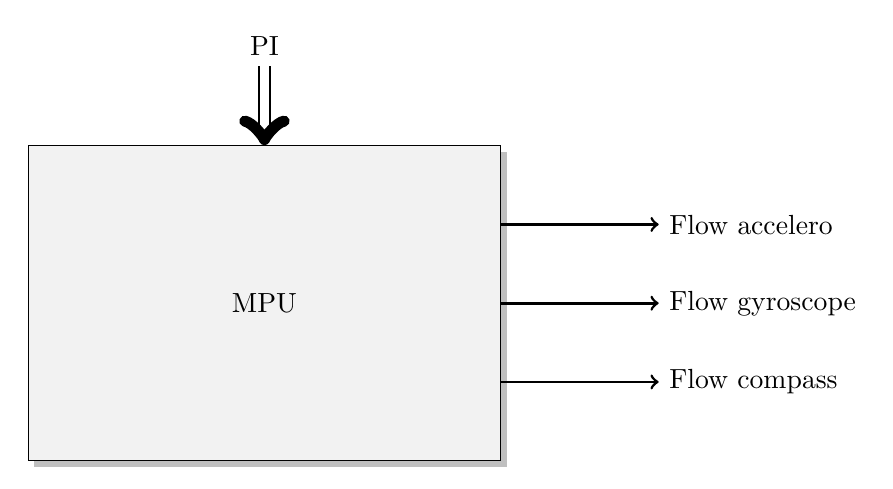
\begin{tikzpicture}[scale=2]
\node[block,rectangle,minimum height=4cm,minimum width=6cm] (bloc) {MPU};
\path[connect,->] (bloc.east) -- ++ (1cm,0) node[right]{Flow gyroscope};
\path[connect,->] ([yshift=0.5cm]bloc.east) -- ++ (1cm,0) node[right]{Flow accelero};
\path[connect,->] ([yshift=-0.5cm]bloc.east) -- ++ (1cm,0) node[right]{Flow compass};
\path[connect,<-][double distance = 3pt] (bloc.north)  -- ++(0,0.5cm) node[above]{PI};
\end{tikzpicture}



\end{document}